%%%%%%%%%%%%%%%%%%%%%%%%%%%%%%%%%%%%%%%%%%%%%%%%%%%%%%%%%%%%%%%%%%%%%%%%%%%%%%%%
%2345678901234567890123456789012345678901234567890123456789012345678901234567890
%        1         2         3         4         5         6         7         8

\documentclass[letterpaper, 10 pt, conference]{ieeeconf}  % Comment this line out if you need a4paper

%\documentclass[a4paper, 10pt, conference]{ieeeconf}      % Use this line for a4 paper

\IEEEoverridecommandlockouts                              % This command is only needed if 
                                                          % you want to use the \thanks command

\overrideIEEEmargins                                      % Needed to meet printer requirements.

%In case you encounter the following error:
%Error 1010 The PDF file may be corrupt (unable to open PDF file) OR
%Error 1000 An error occurred while parsing a contents stream. Unable to analyze the PDF file.
%This is a known problem with pdfLaTeX conversion filter. The file cannot be opened with acrobat reader
%Please use one of the alternatives below to circumvent this error by uncommenting one or the other
%\pdfobjcompresslevel=0
%\pdfminorversion=4

% See the \addtolength command later in the file to balance the column lengths
% on the last page of the document

% The following packages can be found on http:\\www.ctan.org
\usepackage{graphics} % for pdf, bitmapped graphics files
\usepackage{epsfig} % for postscript graphics files
\usepackage{mathptmx} % assumes new font selection scheme installed
\usepackage{times} % assumes new font selection scheme installed
\usepackage{amsmath} % assumes amsmath package installed
\usepackage{amssymb}  % assumes amsmath package installed
\usepackage[latin1]{inputenc}

% Bildumgebungen
\usepackage{graphicx}
\graphicspath{{picture/}}
% \usepackage{import}
\usepackage{xcolor}
\usepackage{tabularx}

\usepackage{blindtext}
\usepackage{url}

% for tables
\usepackage{booktabs}


\title{\LARGE \bf
Developement of an autonomous driving environment model visualization based on object list level
}


\author{Tobias Wagner  Christoph Zach Max Haindl Philipp Korn Stehpan ...? Dennis Roessler Max Pfaller Domi ...? % <-this % stops a space
\thanks{*This work was not supported by any organization}% <-this % stops a space
}


\begin{document}



\maketitle
\thispagestyle{empty}
\pagestyle{empty}


%%%%%%%%%%%%%%%%%%%%%%%%%%%%%%%%%%%%%%%%%%%%%%%%%%%%%%%%%%%%%%%%%%%%%%%%%%%%%%%%
\begin{abstract}

This electronic document is a live template. The various components of your paper [title, text, heads, etc.] are already defined on the style sheet, as illustrated by the portions given in this document.

\end{abstract}


%%%%%%%%%%%%%%%%%%%%%%%%%%%%%%%%%%%%%%%%%%%%%%%%%%%%%%%%%%%%%%%%%%%%%%%%%%%%%%%%
\section{INTRODUCTION}


\section{RELATED WORKS}

IEEE Fabio Reway Test Method for Measuring the Simulation-to-Reality Gap of Camera-based Object Detection Algorithms for Autonomous Driving


\section{MATERIALS AND METHODS}

Kleines Intro was jetzt kommt


\begin{figure}[thpb]
      \centering
       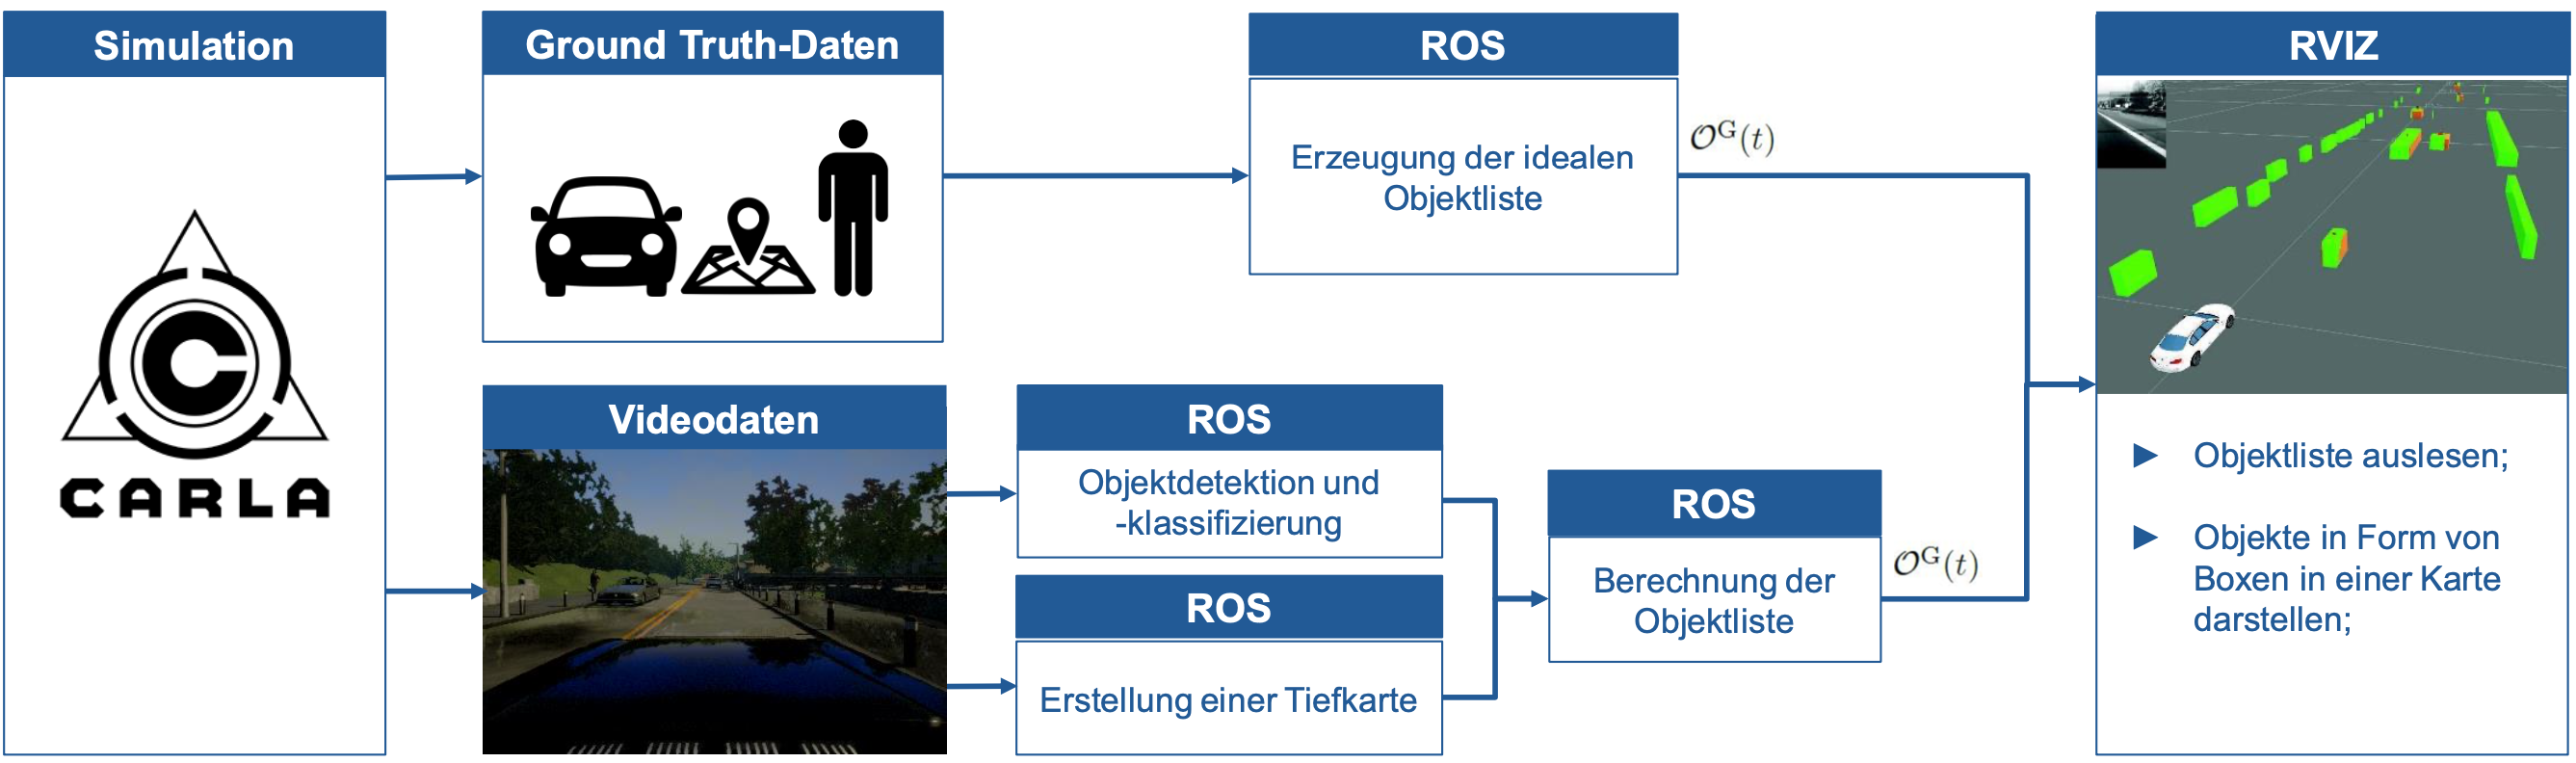
\includegraphics[scale=0.17]{Ueberblick}
      \caption{Ueberblick }
      \label{figurelabel}
   \end{figure}
\subsection{Creating simulation scenario}

\begin{itemize}
\item Welcher Simulator wurde verwendet
\item Welches Szenario (NCAP)
\item Szenario beschreiben
\end{itemize}


   
\subsection{Creating objects list of ground-truth data (TP1}

\begin{itemize}
\item Erstellung Objektliste
\item Objektliste anhand Attribut-Vektor beschreiben
\item Ros-System beschreiben
\item Feature Vektor Ermittlung
\end{itemize}

   \begin{figure}[thpb]
      \centering
       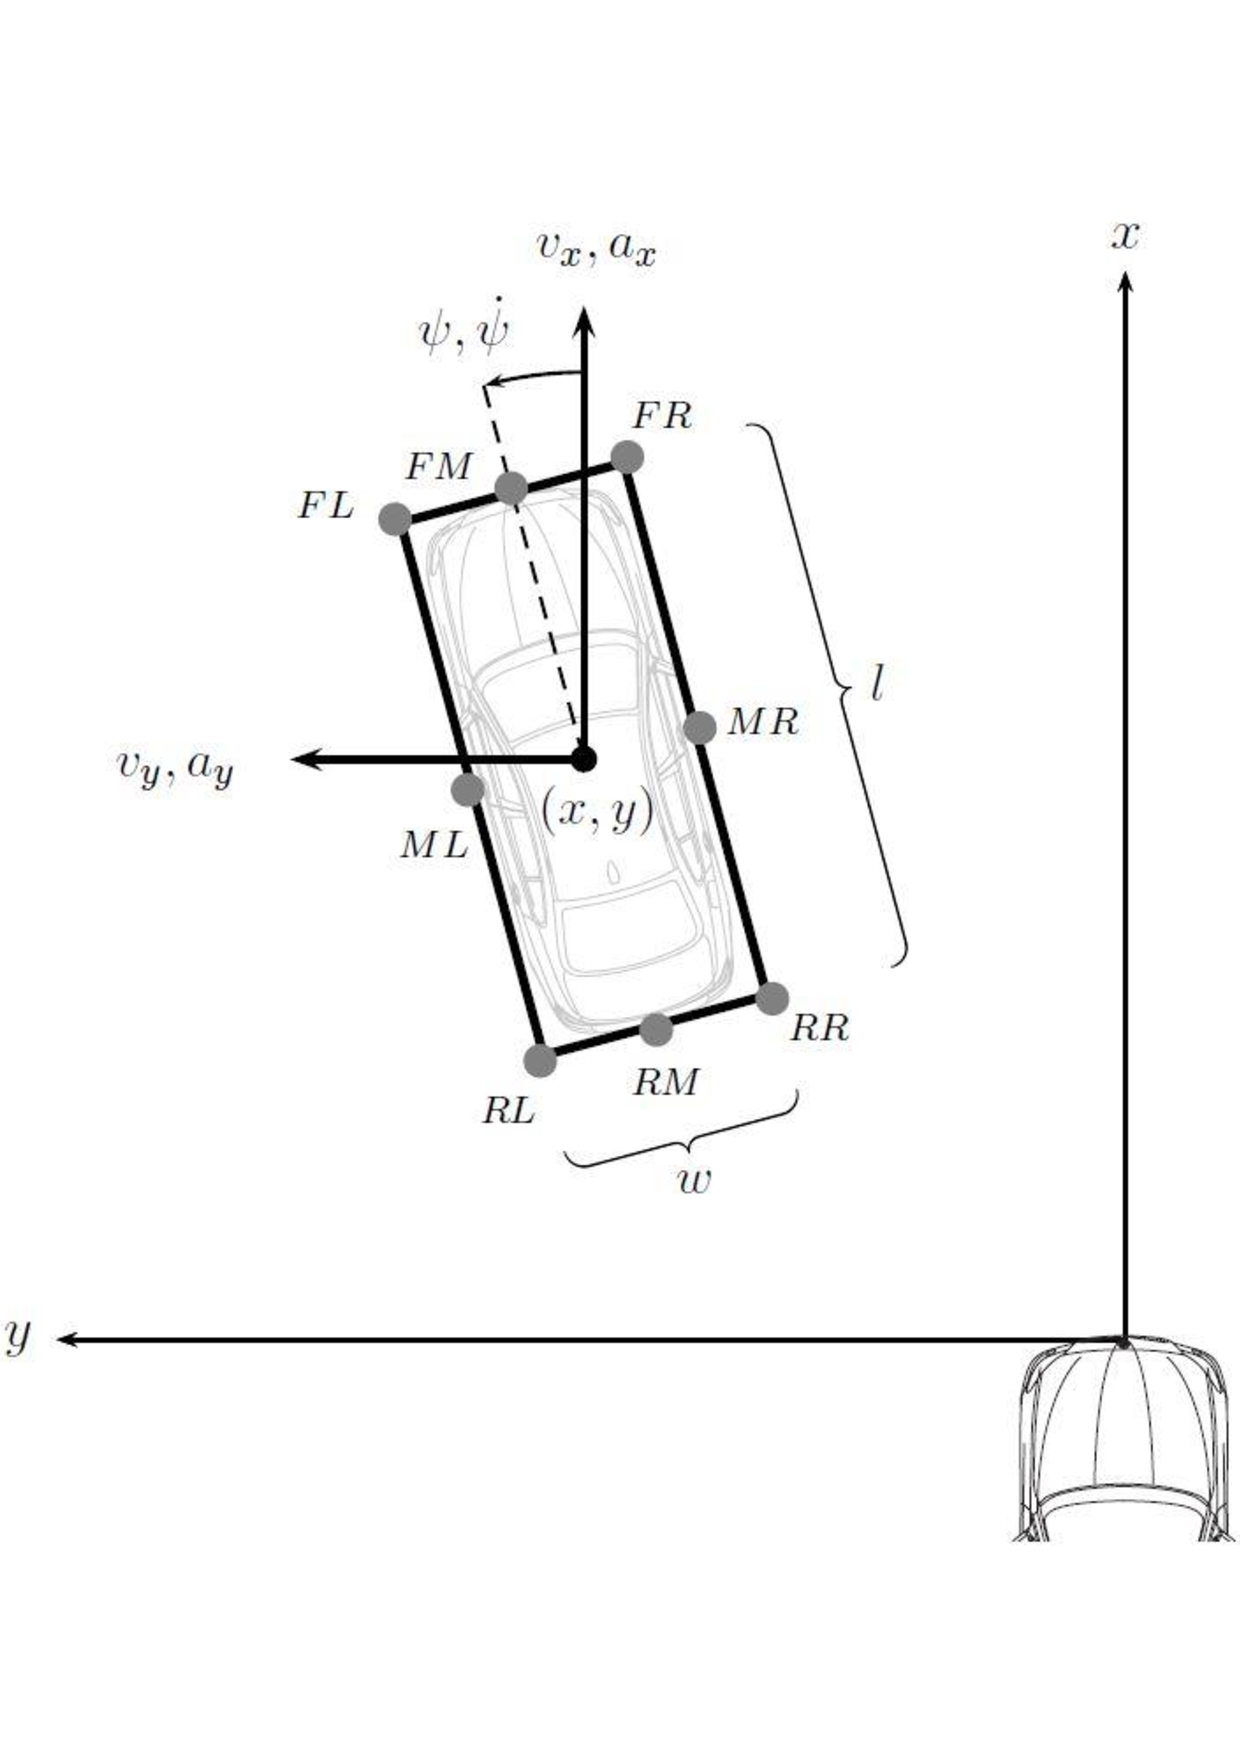
\includegraphics[scale=0.3]{KoordinatenSystem}
      \caption{Fahrzeugkoordinatensystem}
      \label{figurelabel}
   \end{figure}
\subsection{Evaluation of video data (TP2)}

\begin{itemize}
\item Detektion Objekte (Yolo)
\item Tracking Objekte (Tracker)
\item Gleichung zur Berechnung von zB Geschwindigkeit, Beschleunigung
\item Ermittlung Classification / prop mov / prop exis

\end{itemize}


%Die erzeugten Objektlisten aus den groundtruth Daten bzw. Videodaten werden über ROS veröffentlicht. 

\subsection{Visualization of object lists(TP3)}

The published topics of Ground-Truth data and Camera-Calculation data will be subscribed. Each topic contains the ego vehicle data and the specific generated object list. In order to evaluate the object lists, the objects will be analyzed per frame. In RVIZ, the objects are represented by primitive figures with the help of marker messages.



Marker messages are described with specific properties such as position, scale, type, color, orientation. Each object class will assigned selected shapes and colors so that they can be differentiate in RVIZ. The display variants for the possible object classes are shown in table \ref{ClassificationAssignment}. 

\begin{table}[h]
\caption{Classification Assignment}
\label{ClassificationAssignment}
\begin{center}
\begin{tabular}{c c c}
\hline
Classification & Shape & Color[RGB]\\
\hline
car & cube & [1, 0, 0]\\
truck & cube & [0, 1, 0]\\
pedestrian & cylinder & [0, 0, 1]\\
motorcyle & cube & [1, 0, 1]\\
car & cube & [1, 0, 0]\\
bicycle & cylinder & [1, 1, 0]\\
stacionary & sphere & [0, 1, 1]\\
other & sphere & [1, 1, 1]\\
\hline


\end{tabular}
\end{center}
\end{table}

In Addition, the yaw angle of the objects has to be transformed into a quaternion for the visualization in RVIZ. The markers for the calculated camera data are assigned an RGB alpha value of 0.5, so that the difference between the camera data and the GT data is visually recognizable. 

The highest detection probability of an object indicates the classification, so that the properties value of each shape can assigned to the marker message. Furthermore, each detection position must be mirrored on the Y-axis, because the vehicle coordinate system does not match to the RVIZ coordinate system. Finally, the generated markers are combined into a marker array and will be published.

The pubished topics of Ground-Truth data, camera date and ego vehicle data are also saved in a Rosbag File. Each bagfile contains the published ego data and the corresponding object lists.In the following, these files are used for postprocessing.

%%%% IoU calculation %%%%

% necessary packages:
	% \usepackage{booktabs}
	% \usepackage{tabularx}

\subsubsection{Evaluation}
\label{sssec:eval}
To determine whether a given camera object is evaluated as True Positive (TP), False Positive (FP), False Negative (FN) or a mismatch (mm), the \textbf{Intersection over Union} (IoU) value is used, like shown in \cite{Reway}. 
Like shown before, in general there is a list of $m$ camera objects ($B_{pr}$) and a list of $n$ ground truth objects ($B_{gt}$) for each frame. To evaluate a frame, for each combination of GT object and camera object the IoU value is calculated. All those values build a matrix like shown in Table \ref{tab:matrix}.
\begin{table}[h]
	\caption{IoU-Matrix for a single frame}
	\begin{tabularx}{\columnwidth}{X|X|c|X}
		\toprule
		$IoU(B_{gt,1}, B_{pr,1})$ & $IoU(B_{gt,2}, B_{pr,1})$ & ... & $IoU(B_{gt,n}, B_{pr,1})$ \\
		\midrule
		$IoU(B_{gt,1}, B_{pr,2})$ & $IoU(B_{gt,2}, B_{pr,2})$ & ... & $IoU(B_{gt,n}, B_{pr,2})$ \\
		\midrule
		... & ... & ... & ... \\
		\midrule		
		$IoU(B_{gt,1}, B_{pr,m})$ & $IoU(B_{gt,2}, B_{pr,m})$ & ... & $IoU(B_{gt,n}, B_{pr,m})$ \\
		\bottomrule
	\end{tabularx}
	\label{tab:matrix}
\end{table}

A given camera object $B_{pr,i}$ is ... \\

... \textbf{FP}, if there is no value 
\begin{equation}
	IoU(B_{gt,k}, B_{pr,i}) > t \text{\quad with\quad} k \in \left\lbrace 1, ..., n\right\rbrace 
	\label{eq:fp_case}
\end{equation}
in the according row of the matrix which is greater than the given threshold. \\

... \textbf{FP}, if there is one or more IoU values in the according row greater than the threshold, but for every $B_{gt,k}$, for which equation \ref{eq:fp_case} is true, there is another $B_{pr,j}$ ($j\neq i$) which matches with $B_{gt,k}$ and $IoU(B_{gt,k}, B_{pr,j}) > IoU(B_{gt,k}, B_{pr,i})$ \\

... a mismatch (\textbf{mm}) if it is no FP case, but none of the found possible matching $B_{gt,k}$ has the same class as $B_{pr,i}$. \\

... \textbf{TP}, also called a match, if none of the other mentioned cases are detected. That means, that there is at least one $B_{gt,k}$ which fulfills equation \ref{eq:fp_case} and has the same classification as $B_{pr,i}$ and there is no other $B_{pr,j}$ which matches better with the found $B_{gt,k}$ \\

Going through the rows of the matrix, for each $B_{pr,i}$ in the given frame it can be decided, whether the case is TP, FP or mm. \\

On the other way round, examining the Ground Truth objects $B_{gt,k}$, that means the columns of the calculated matrix, all FN cases can be detected. It is an \textbf{FN}, if there is no $B_{pr,i}$ for which
\begin{equation}
IoU(B_{gt,k}, B_{pr,i}) > t \text{\quad with\quad} i \in \left\lbrace 1, ..., m\right\rbrace 
\label{eq:fn_case}
\end{equation}
Going through the columns of the matrix, this decision can be made for every $B_{gt,k}$. \\
With this steps, a given frame with $m$ camera objects and $n$ ground truth objects can be investigated. \\

In this project these functions, one for investigating the camera objects and one for detecting all FN cases, were realized in Python. The calculation of an IoU value is processed with functions of the package \textit{shapely} \cite{Shapely}.
First, the given objects, which are defined through their properties \textit{x}, \textit{y}, \textit{length}, \textit{height}, \textit{yaw} and \textit{classification} like presented in \cite{Aeberhard}
are transformed into bounding boxes with a shapely function. With two of these bounding boxes shapely can calculate the intersection area and the union area, and so the IoU value can be processed. \\

\subsubsection{Graphical User Interface}
To investigate the quality of the processed camera object data, a graphical user interface (GUI) was created. It was designed with Pythons binding package for Qt (PyQt5) \cite{PyQt}
and defined as a plugin for \textit{rqt}, a \textit{ROS} framework for GUI development \cite{rqt}.
With this plugin, the user can import two bag files, one ground truth data bag file and one camera data bag file.
By using the functions mentioned before, the GUI can show several data graphs to the user, like raw data plots, comparing plots with object data of both files or evaluation data. 
% TODO: mit Christophs Bezeichnungen vergleichen
Along with the data the mean value and the standard deviation for each data set is portrayed in the GUI. \\
Apart from data plots the interface can also show quality parameters for the whole camera data bag file in an extra widget. 
% TODO: Verweis auf Christophs part
For each operation, where IoU calculation is needed, the user can set the threshold value for the evaluation. \\

\subsubsection{Results}
% TODO: in Kapitel RESULTS kopieren
% TODO: Auswerten
	% Vorausgehende Beschreibung der Situation
	% Wie viele Objekte werden erkannt?
	% Wie viele Objekte werden gematcht?
		% evtl. vergleichende Tabelle bei verschiedenen Threshold-Werten
		% Tabellen mit FPPI, MOTP, MOTA bei versch. Threshold-Werten
The performance of processed camera data can be evaluated with metrics presented in \cite{Reway}, which are realized like introduced in part \ref{sssec:eval}. For the given scenario the reached performance is shown in Table \ref{tab:res}.
		
\begin{table}[h]
	\caption{Performance results}
	\begin{tabularx}{\columnwidth}{XXXX}
		\toprule
		\textbf{threshold} & $t=0.5$ & $t=0.6$ & $t=0.7$ \\
		\toprule
		Precision & ... & ... & ... \\
		\midrule
		Recall & ... & ... & ... \\
		\midrule		
		FPPI & ... & ... & ... \\
		\midrule
		MOTA & ... & ... & ... \\
		\midrule
		MOTP & ... & ... & ... \\
		\bottomrule
	\end{tabularx}
	\label{tab:res}
\end{table}
		
\subsubsection{Conclusions}
% TODO: in Kapitel CONCLUSIONS kopieren
% Werte schlecht, weil z.B. die geometric und dimension Werte der Kamera nicht gut mit den GT-Daten übereinstimmen
	



 



\section{RESULTS}

Ergebnisse des Projekts:
 
 \begin{itemize}
\item Funktioniert die Auswertung
\item Wie gut sind die Kamerawerte im Vergleich zu Groundtruth Werte
\item sind die Werte represenativ
\end{itemize}

   
\section{CONCLUSIONS}



\addtolength{\textheight}{-12cm}   % This command serves to balance the column lengths
                                  % on the last page of the document manually. It shortens
                                  % the textheight of the last page by a suitable amount.
                                  % This command does not take effect until the next page
                                  % so it should come on the page before the last. Make
                                  % sure that you do not shorten the textheight too much.


\section*{APPENDIX}



\section*{ACKNOWLEDGMENT}



\bibliographystyle{IEEEtran}{
\bibliography{ref/ref_list.bib}}


\end{document}
